Welcome to week 3! This week, we’ll be covering logistic regression. Logistic regression is a method for classifying data into discrete outcomes. For example, we might use logistic regression to classify an email as spam or not spam. In this module, we introduce the notion of classification, the cost function for logistic regression, and the application of logistic regression to multi-class classification.

We are also covering regularization. Machine learning models need to generalize well to new examples that the model has not seen in practice. We’ll introduce regularization, which helps prevent models from overfitting the training data. 

\section{Classification and Representation}
\subsection{Hypothesis Representation}
In binary classification problem, output $y$ will only be $0$ or $1$. Using linear regression and a threshold to determine where $y = 1$ or $y = 0$ because some extreme input data can modify brutally the regression. Therefore, we need to use another hypothesis function, the \textbf{Sigmoid Function} (also called \textbf{Logistic Function}) which is defined in formula \eqref{formSigmoid}.
\begin{align} \label{formSigmoid}
	h_\theta (x) 	&=  g ( \theta^T x ) \nonumber \\
	z 				&= \theta^T x \nonumber \\
	g(z) 			&= \dfrac{1}{1 + e^{-z}}
\end{align}
\myaligns{Sigmoid Function}
The code in listing \ref{lstSigmoid} shows how to plot this function (figure \ref{figSigmoid}) in Octave.
\lstinputlisting[label=lstSigmoid,caption=Sigmoid Function]{./week3/sigmoidPlot.m}
The function $g(z)$, shown here, maps any real number to the $(0, 1)$ interval, making it useful for transforming an arbitrary-valued function into a function better suited for classification. We start with our old hypothesis (linear regression), except that we want to restrict the range to 0 and 1. This is accomplished by plugging $z = \theta^Tx$ into the Logistic Function. 
\begin{figure}[!ht]
\centering
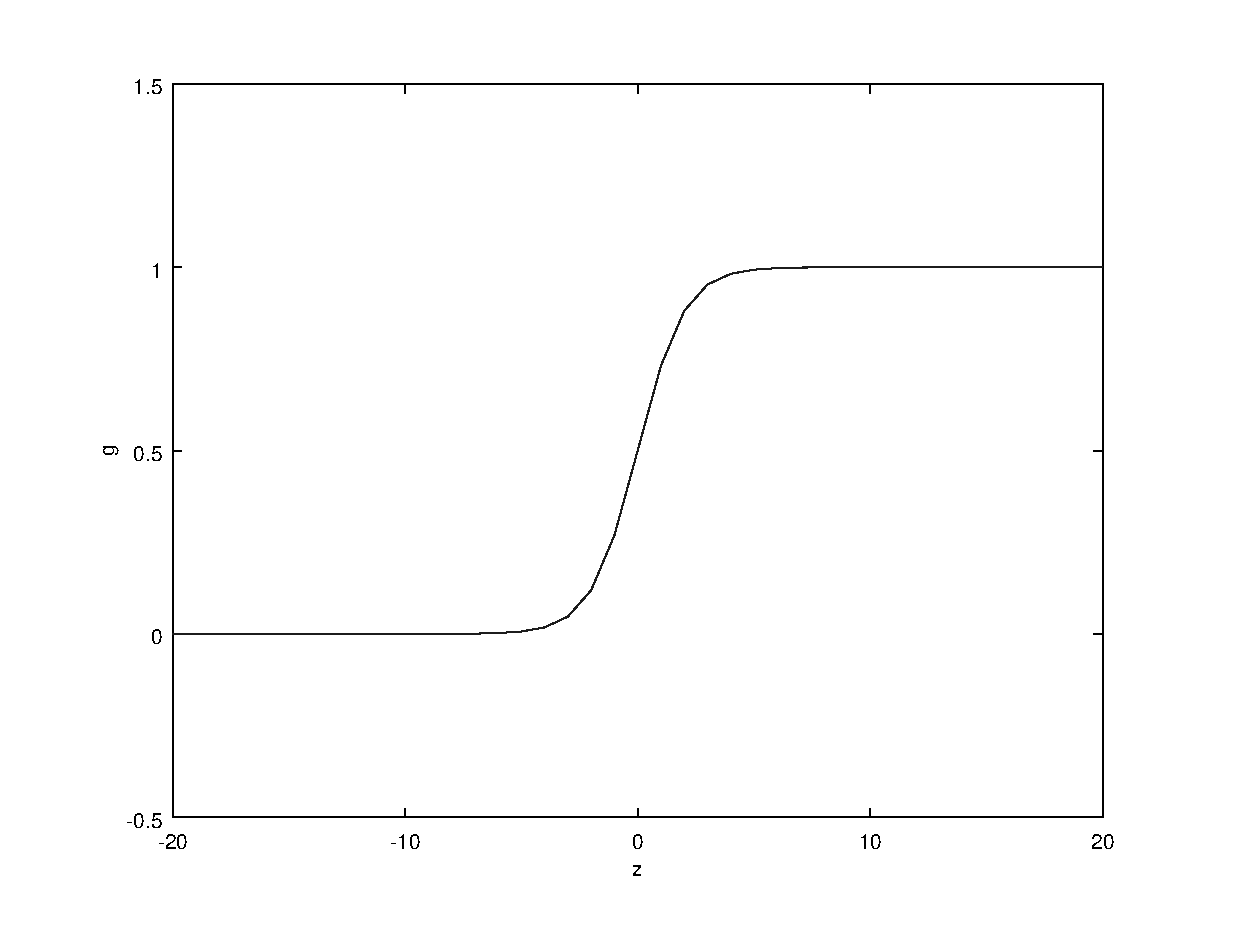
\includegraphics[scale = 0.6]{sigmoid.eps}
\caption[Sigmoid Function]{Sigmoid Function: $g = \frac{1}{1 + e^{-z}}$}
\label{figSigmoid}
\end{figure}

\subsection{Boundary Decision}
The hypothesis function $h_\theta$ gives us the probability that our output equals $1$. In binary classification, we have:
\begin{align*}
h_\theta(x) &= \mathbb{P}(y=1 | x ; \theta) = 1 - \mathbb{P}(y=0 | x ; \theta)
\end{align*} 
In order to get our discrete 0 or 1 classification, we can translate the output of the hypothesis function as follows:
\begin{align*}
& h_\theta(x) \geq 0.5 \rightarrow y = 1 \\
& h_\theta(x) < 0.5 \rightarrow y = 0
\end{align*}
From formula \eqref{formSigmoid} we deduce that:
\begin{align*}
h_\theta(x) = g(\theta^T x) \geq 0.5 \Leftrightarrow \theta^T x \geq 0
\end{align*}
which is equivalent to expression below: 
\begin{align}
& \theta^T x \geq 0 \rightarrow y = 1 \\
& \theta^T x < 0 \rightarrow y = 0 \nonumber
\end{align}
The \textbf{Boundary Decision} is the line separates the two areas $y = 0$ and $y = 1$. It can be a straight line or a circle and so on. In fact, it's the set of $x$ that satisfying formula \eqref{formBounDeci}:
\begin{align} \label{formBounDeci}
\theta^Tx = 0
\end{align}
\myaligns{Boundary Decision}

\section{Logistic Regression Model}

\subsection{Cost Function}
We cannot use the same cost function declared in \eqref{form:matCostFunc} (which aims to reduce the mean squared error) because the logistic function $h_\theta(x)$ will cause the cost function $J(\theta)$ to be wavy, i.e. not a convex function hence difficult to compute global optimization. Recall that cost function $J(\theta)$ can be written as following:
\begin{align}
J(\theta) = \dfrac{1}{m} \sum_{i=1}^m \mathrm{Cost}(h_\theta(x^{(i)}),y^{(i)})
\end{align}
In which, \textbf{Maximum Likelihood Estimation} will lead us to $\mathrm{Cost}(h_\theta(x^{(i)}),y^{(i)})$ defined in formula \eqref{formCostFuncLogisElem}. Note that $y$ only takes value $0$ or $1$.
\begin{align} \label{formCostFuncLogisElem}
\mathrm{Cost}(h_\theta(x),y) = - y \; \log(h_\theta(x)) - (1 - y) \log(1 - h_\theta(x))
\end{align}
\myaligns{$\mathrm{Cost}(h_\theta(x^{(i)}),y^{(i)})$ in Logistic Regression}

From figure \ref{figCostLogisticPlot}, the more our hypothesis is off from $y$, the larger the cost function output. If our hypothesis is equal to $y$, then our cost is $0$.
\begin{figure}[!ht]
\centering
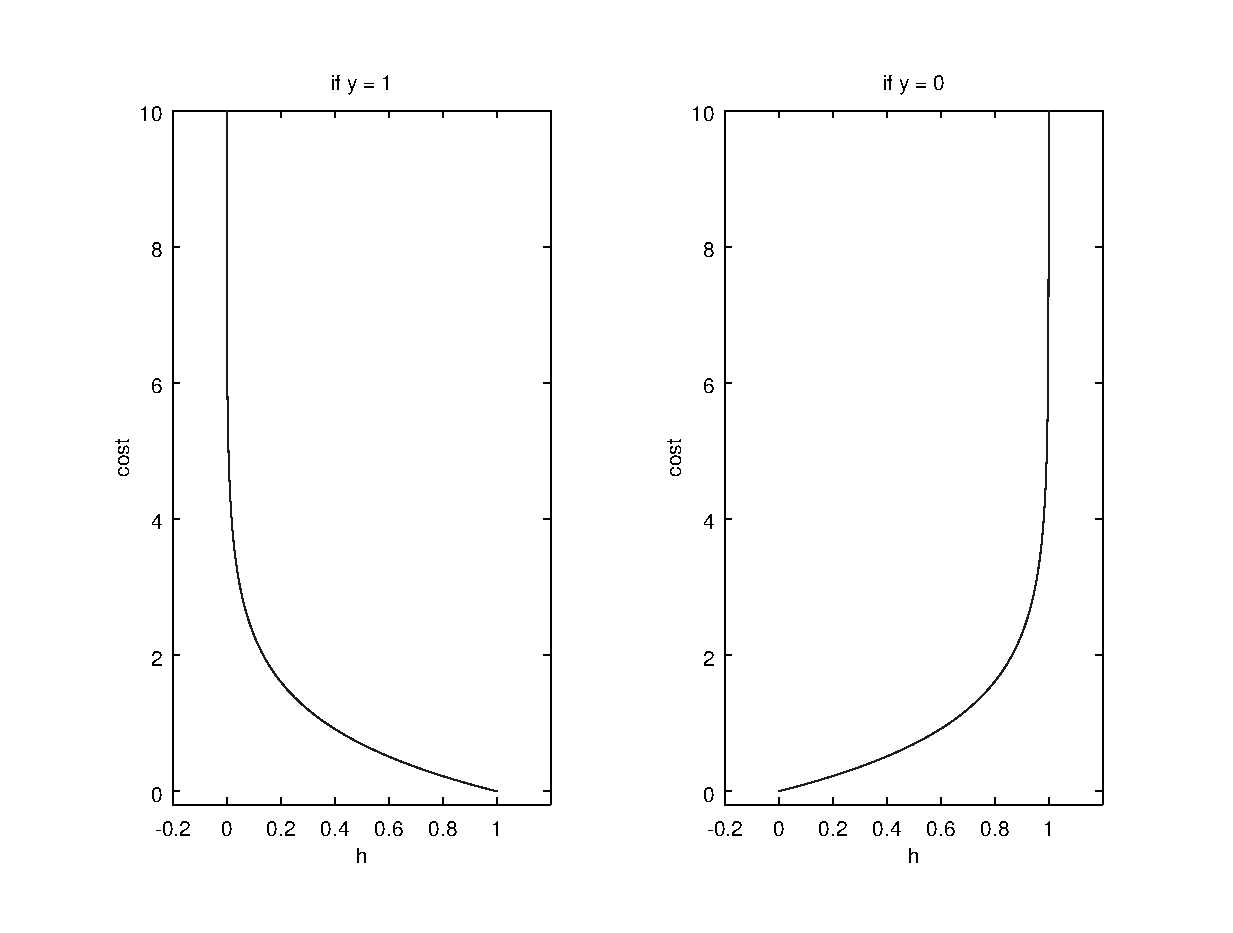
\includegraphics[scale = 0.7]{costLogisticPlot.eps}
\caption[Cost Function in Logistic Regression]{Cost Function in Logistic Regression: the more our hypothesis is off from $y$, the larger the cost function output. If our hypothesis is equal to $y$, then our cost is $0$.}
\label{figCostLogisticPlot}
\end{figure}

\subsection{Gradient Descent for Logistic Regression}
We can fully write our entire cost function as follows:
\begin{align}\label{formCostFuncLogis}
J(\theta) = - \frac{1}{m} \sum_{i=1}^m [y^{(i)}\log (h_\theta (x^{(i)})) + (1 - y^{(i)})\log (1 - h_\theta(x^{(i)}))]
\end{align}

We want compute its partial derivatives to $\theta$ in order to use Gradient Descent. I recall here some derivatives used here:
\begin{align}
log(u(\theta))' 								&= \frac{u'(\theta)}{u(\theta)} \\
(\frac{1}{u(\theta)})' 							&= \frac{-u'(\theta)}{u^2(\theta)} \\
\frac{\partial}{\partial \theta} e^{-\theta^Tx} &= -e^{-\theta^Tx}x
\end{align}  

In our case, we have the following facts:
\begin{align}
h_\theta(x) 									&= g(\theta^Tx) = \frac{1}{1 + e^{-\theta^Tx}} \\
1 - h_\theta(x) 	&= e^{-\theta^Tx}h_\theta(x) \\
\frac{\partial}{\partial \theta} h_\theta(x) 	&= -e^{-\theta^Tx}(h_\theta(x))^2 x
\end{align}

Applying derivatives in formula \eqref{formCostFuncLogis}, we have the gradient of $J(\theta)$ as follows:
\begin{align*} 
\frac{\partial}{\partial \theta_j} J(\theta) = \frac{1}{m}\sum_{i=1}^m \left [ h_\theta(x^{(i)}) - y^{(i)} \right ] x^{(i)}_j
\end{align*}

Hence, Gradient Descent for Logistic Regression is:
\begin{align}\label{formGradDescExpli}
\theta_j := \theta_j - \alpha \frac{1}{m} \sum_{i=1}^m (h_\theta(x^{(i)}) - y^{(i)}) x_j^{(i)}
\end{align}

Note that this gradient descent form of $\theta$ is the same as in Linear Regression (formula \eqref{form:w2mulVarGradDesc}). Formula \eqref{formGradDescExpli} can also be expressed in matrix form as follows:
\begin{align}\label{formGradDescMat}
\theta := \theta - \frac{\alpha}{m} X^T (g(X\theta) - y) = \theta - \frac{\alpha}{m} X^T (\frac{1}{1 + e^{-X\theta}} - y)
\end{align}
\myaligns{Gradient Descent of Logistic Regression}
We can see that: 
\begin{itemize}
	\item in Linear Regression: $g(X\theta) = X\theta$ is a linear function
	\item in Logistic Regression: $g(X\theta) = \frac{1}{1 + e^{-X\theta}}$ is a sigmoid function
\end{itemize}

The vectorized form of cost function can be expressed in formula \eqref{formCostFuncLogisMat} below.
\begin{align} \label{formCostFuncLogisMat}
J\left(\theta\right)  =  -\frac{1}{m}\left(\log\left(g\left(X\theta\right)\right)^{T}y+\log\left(1-g\left(X\theta\right)\right)^{T}\left(1-y\right)\right)
\end{align}
\myaligns{Vectorization of Logistic Cost Function}


\subsection{Advanced Optimization in Octave}
\textbf{Conjugate Gradient}, \textbf{BFGS}, and \textbf{L-BFGS} are more sophisticated, faster ways to optimize theta instead of using gradient descent. Prof. A. Ng suggests you do not write these more sophisticated algorithms yourself (unless you are an expert in numerical computing) but use them pre-written from libraries. Octave provides them once we define a cost function $J(\theta)$ and its gradient $\dfrac{\partial}{\partial \theta_j}J(\theta), \; j=0,..,n+1$. We can apply vectorization on gradient of $J(\theta)$ if possible since it avoids duplicating code. An example is shown in listing \ref{lstFminuncExp} using a cost function $J = (\theta_1 - 5)^2 + (\theta_2 - 5)^2$ defined in listing \ref{lstCostFunc}.
\lstinputlisting[caption=Octave \textbf{fminunc} example, label=lstFminuncExp]{week3/fminuncExample.m}
\lstinputlisting[caption=Cost Function, label=lstCostFunc]{week3/costFunction.m}


\section{Multi-class Classification}
If we have more than 2 classes, we can repeatedly use Binary Classification by separating all classes to one single class and the rest. Mathematically, if we have $n + 1$ classes $y \in \lbrace0, 1 ... n\rbrace$, then, we divide the problem into $n+1$ binary classification where we predict the probability that $y$ is in that single class. This problem is declared below:
\begin{align*}
& y \in \lbrace0, 1 ... n\rbrace \\
& h_\theta^{(0)}(x) = P(y = 0 | x ; \theta) \\
& h_\theta^{(1)}(x) = P(y = 1 | x ; \theta) \\
& \cdots \\
& h_\theta^{(n)}(x) = P(y = n | x ; \theta) \\
& \mathrm{prediction} = \max_i( h_\theta ^{(i)}(x) )\\
\end{align*}
Given a new input, we use the hypothesis that returns the highest probability as our prediction.

\section{Regularization}
\subsection{The Problem of Overfitting}
